% Options for packages loaded elsewhere
\PassOptionsToPackage{unicode}{hyperref}
\PassOptionsToPackage{hyphens}{url}
%
\documentclass[
  11pt,
]{article}
\usepackage{lmodern}
\usepackage{setspace}
\usepackage{amssymb,amsmath}
\usepackage{ifxetex,ifluatex}
\ifnum 0\ifxetex 1\fi\ifluatex 1\fi=0 % if pdftex
  \usepackage[T1]{fontenc}
  \usepackage[utf8]{inputenc}
  \usepackage{textcomp} % provide euro and other symbols
\else % if luatex or xetex
  \usepackage{unicode-math}
  \defaultfontfeatures{Scale=MatchLowercase}
  \defaultfontfeatures[\rmfamily]{Ligatures=TeX,Scale=1}
  \setmainfont[]{Carlito}
\fi
% Use upquote if available, for straight quotes in verbatim environments
\IfFileExists{upquote.sty}{\usepackage{upquote}}{}
\IfFileExists{microtype.sty}{% use microtype if available
  \usepackage[]{microtype}
  \UseMicrotypeSet[protrusion]{basicmath} % disable protrusion for tt fonts
}{}
\makeatletter
\@ifundefined{KOMAClassName}{% if non-KOMA class
  \IfFileExists{parskip.sty}{%
    \usepackage{parskip}
  }{% else
    \setlength{\parindent}{0pt}
    \setlength{\parskip}{6pt plus 2pt minus 1pt}}
}{% if KOMA class
  \KOMAoptions{parskip=half}}
\makeatother
\usepackage{xcolor}
\IfFileExists{xurl.sty}{\usepackage{xurl}}{} % add URL line breaks if available
\IfFileExists{bookmark.sty}{\usepackage{bookmark}}{\usepackage{hyperref}}
\hypersetup{
  hidelinks,
  pdfcreator={LaTeX via pandoc}}
\urlstyle{same} % disable monospaced font for URLs
\usepackage[margin=15mm]{geometry}
\usepackage{color}
\usepackage{fancyvrb}
\newcommand{\VerbBar}{|}
\newcommand{\VERB}{\Verb[commandchars=\\\{\}]}
\DefineVerbatimEnvironment{Highlighting}{Verbatim}{commandchars=\\\{\}}
% Add ',fontsize=\small' for more characters per line
\usepackage{framed}
\definecolor{shadecolor}{RGB}{248,248,248}
\newenvironment{Shaded}{\begin{snugshade}}{\end{snugshade}}
\newcommand{\AlertTok}[1]{\textcolor[rgb]{0.94,0.16,0.16}{#1}}
\newcommand{\AnnotationTok}[1]{\textcolor[rgb]{0.56,0.35,0.01}{\textbf{\textit{#1}}}}
\newcommand{\AttributeTok}[1]{\textcolor[rgb]{0.77,0.63,0.00}{#1}}
\newcommand{\BaseNTok}[1]{\textcolor[rgb]{0.00,0.00,0.81}{#1}}
\newcommand{\BuiltInTok}[1]{#1}
\newcommand{\CharTok}[1]{\textcolor[rgb]{0.31,0.60,0.02}{#1}}
\newcommand{\CommentTok}[1]{\textcolor[rgb]{0.56,0.35,0.01}{\textit{#1}}}
\newcommand{\CommentVarTok}[1]{\textcolor[rgb]{0.56,0.35,0.01}{\textbf{\textit{#1}}}}
\newcommand{\ConstantTok}[1]{\textcolor[rgb]{0.00,0.00,0.00}{#1}}
\newcommand{\ControlFlowTok}[1]{\textcolor[rgb]{0.13,0.29,0.53}{\textbf{#1}}}
\newcommand{\DataTypeTok}[1]{\textcolor[rgb]{0.13,0.29,0.53}{#1}}
\newcommand{\DecValTok}[1]{\textcolor[rgb]{0.00,0.00,0.81}{#1}}
\newcommand{\DocumentationTok}[1]{\textcolor[rgb]{0.56,0.35,0.01}{\textbf{\textit{#1}}}}
\newcommand{\ErrorTok}[1]{\textcolor[rgb]{0.64,0.00,0.00}{\textbf{#1}}}
\newcommand{\ExtensionTok}[1]{#1}
\newcommand{\FloatTok}[1]{\textcolor[rgb]{0.00,0.00,0.81}{#1}}
\newcommand{\FunctionTok}[1]{\textcolor[rgb]{0.00,0.00,0.00}{#1}}
\newcommand{\ImportTok}[1]{#1}
\newcommand{\InformationTok}[1]{\textcolor[rgb]{0.56,0.35,0.01}{\textbf{\textit{#1}}}}
\newcommand{\KeywordTok}[1]{\textcolor[rgb]{0.13,0.29,0.53}{\textbf{#1}}}
\newcommand{\NormalTok}[1]{#1}
\newcommand{\OperatorTok}[1]{\textcolor[rgb]{0.81,0.36,0.00}{\textbf{#1}}}
\newcommand{\OtherTok}[1]{\textcolor[rgb]{0.56,0.35,0.01}{#1}}
\newcommand{\PreprocessorTok}[1]{\textcolor[rgb]{0.56,0.35,0.01}{\textit{#1}}}
\newcommand{\RegionMarkerTok}[1]{#1}
\newcommand{\SpecialCharTok}[1]{\textcolor[rgb]{0.00,0.00,0.00}{#1}}
\newcommand{\SpecialStringTok}[1]{\textcolor[rgb]{0.31,0.60,0.02}{#1}}
\newcommand{\StringTok}[1]{\textcolor[rgb]{0.31,0.60,0.02}{#1}}
\newcommand{\VariableTok}[1]{\textcolor[rgb]{0.00,0.00,0.00}{#1}}
\newcommand{\VerbatimStringTok}[1]{\textcolor[rgb]{0.31,0.60,0.02}{#1}}
\newcommand{\WarningTok}[1]{\textcolor[rgb]{0.56,0.35,0.01}{\textbf{\textit{#1}}}}
\usepackage{longtable,booktabs}
% Correct order of tables after \paragraph or \subparagraph
\usepackage{etoolbox}
\makeatletter
\patchcmd\longtable{\par}{\if@noskipsec\mbox{}\fi\par}{}{}
\makeatother
% Allow footnotes in longtable head/foot
\IfFileExists{footnotehyper.sty}{\usepackage{footnotehyper}}{\usepackage{footnote}}
\makesavenoteenv{longtable}
\usepackage{graphicx,grffile}
\makeatletter
\def\maxwidth{\ifdim\Gin@nat@width>\linewidth\linewidth\else\Gin@nat@width\fi}
\def\maxheight{\ifdim\Gin@nat@height>\textheight\textheight\else\Gin@nat@height\fi}
\makeatother
% Scale images if necessary, so that they will not overflow the page
% margins by default, and it is still possible to overwrite the defaults
% using explicit options in \includegraphics[width, height, ...]{}
\setkeys{Gin}{width=\maxwidth,height=\maxheight,keepaspectratio}
% Set default figure placement to htbp
\makeatletter
\def\fps@figure{htbp}
\makeatother
\setlength{\emergencystretch}{3em} % prevent overfull lines
\providecommand{\tightlist}{%
  \setlength{\itemsep}{0pt}\setlength{\parskip}{0pt}}
\setcounter{secnumdepth}{5}
\usepackage{titling}
\usepackage{multirow}
\usepackage{float}
\let\origfigure\figure
\let\endorigfigure\endfigure
\renewenvironment{figure}[1][2] {
    \expandafter\origfigure\expandafter[H]
} {
    \endorigfigure
}
\pretitle{%
  \begin{center}
  \LARGE
  \includegraphics[width=200mm]{logos.png}\\[\bigskipamount]
}
\posttitle{\end{center}}
\usepackage{booktabs}
\usepackage{longtable}
\usepackage{array}
\usepackage{multirow}
\usepackage{wrapfig}
\usepackage{float}
\usepackage{colortbl}
\usepackage{pdflscape}
\usepackage{tabu}
\usepackage{threeparttable}
\usepackage{threeparttablex}
\usepackage[normalem]{ulem}
\usepackage{makecell}
\usepackage{xcolor}

\title{Future Social Services Institute\\
Visualising the Victorian Care Sector}
\author{Xuejiao Zhou and Ben Cole\\
s3741909 and s3412349}
\date{13 / 06 / 2020}

\begin{document}
\maketitle

{
\setcounter{tocdepth}{2}
\tableofcontents
}
\setstretch{1.1}
\newpage
\setstretch{1.35}

\hypertarget{executive-summary}{%
\section*{Executive Summary}\label{executive-summary}}
\addcontentsline{toc}{section}{Executive Summary}

\hypertarget{acknowledgement}{%
\subsection*{Acknowledgement}\label{acknowledgement}}
\addcontentsline{toc}{subsection}{Acknowledgement}

\hypertarget{declaration-of-originality}{%
\subsection*{Declaration of Originality}\label{declaration-of-originality}}
\addcontentsline{toc}{subsection}{Declaration of Originality}

\hypertarget{glossary}{%
\subsection*{Glossary}\label{glossary}}
\addcontentsline{toc}{subsection}{Glossary}

\hypertarget{student-contributions}{%
\subsection*{Student Contributions}\label{student-contributions}}
\addcontentsline{toc}{subsection}{Student Contributions}

Both student members of the project development team have contributed to the project equally.

\begin{table}[H]
\centering\begingroup\fontsize{10}{12}\selectfont

\begin{tabular}{|>{\raggedright\arraybackslash}p{80mm}|>{\raggedright\arraybackslash}p{40mm}|}
\hline
\rowcolor[HTML]{caf6f9}  \textbf{Section} & \textbf{Contributing Students}\\
\hline
\rowcolor{gray!6}  1 Introduction, 1.1 Background, 1.2 Significance & Ben Cole\\
\hline
2 Brief Literature Review, 2.1 Transformation of the Social Services Sector & Ben Cole\\
\hline
\rowcolor{gray!6}  2.2 Data Visualisations in the Social Care Sector & Xuejiao Zhou\\
\hline
3 Objectives & Xuejiao Zhou\\
\hline
\rowcolor{gray!6}  4 Proposed Methodology, 4.1 Digital Report, 4.2 Visualisation Platform, 4.3 Stakeholder Engagement Workshops & Ben Cole\\
\hline
5 Project Design, 5.1 Timeline & Xuejiao Zhou\\
\hline
\rowcolor{gray!6}  5.2 Collaboration Plan & Ben Cole\\
\hline
6 References & Xuejiao Zhou and Ben Cole\\
\hline
\rowcolor{gray!6}  7 Appendices & Xuejiao Zhou and Ben Cole\\
\hline
\end{tabular}
\endgroup{}
\end{table}

\twocolumn

\hypertarget{introduction}{%
\section{Introduction}\label{introduction}}

The Future Social Services Institute (hereon \emph{FSSI}) has been established cooperatively between the Victorian state government, the Victorian Council of Social Service (\emph{VCOSS}), and the Royal Melbourne Institute of Technology (\emph{RMIT}). The objectives of FSSI are wide-reaching, including (but not limited to) designing educational programs, assisting in workplace training, researching reforms for the social services sector, and supporting transformation in not-for-profit organisations. (Glanz, 2016)

There are numerous industries involved in social services, and these industries can differ between countries and cultures. As this project focuses on the social services in Victoria - and more broadly Australia - the Australian federal government website for the Department of Social Services includes the following sectors:

\begin{itemize}
\tightlist
\item
  Communities and Vulnerable People
\item
  Disability and Carers
\item
  Families and Children
\item
  Housing Support
\item
  Mental Health
\item
  Seniors
\item
  Women's Safety
\item
  Working Age
\item
  Welfare Reform
\end{itemize}

(Department of Social Services, 2019)

In the Victorian government specifically, social services are bundled together with health, but include services operating in areas such as:

\begin{itemize}
\tightlist
\item
  Ageing
\item
  Alcohol and drugs
\item
  Children and families
\item
  Disability
\item
  Housing and homelessness
\item
  Mental health
\end{itemize}

(Department of Health and Social Services, 2019)

\newpage

More broadly, the Australian Association of Social Workers supports the definition of social work as laid out by the International Federation of Social Workers that:

\begin{quote}
\emph{Social work is a practice-based profession and an academic discipline that promotes social change and development, social cohesion, and the empowerment and liberation of people. Principles of social justice, human rights, collective responsibility and respect for diversities are central to social work. Underpinned by theories of social work, social sciences, humanities and indigenous knowledge, social work engages people and structures to address life challenges and enhance wellbeing.}\\
\quad - International Federation of Social Workers, \newline \quad \quad ~~July 2014
\end{quote}

Whilst definitions for which industries comprise social services, the reasons for establishing FSSI and their data needs are much clearer.

\hypertarget{background}{%
\subsection{Background}\label{background}}

\hypertarget{an-ageing-population}{%
\subsubsection{An Ageing Population}\label{an-ageing-population}}

According to the Australian Institute of Health and Welfare, the number of Australians aged 65 and over has been increasing steadily since 1927. In 2017, the total number of Australians over the age of 65 made up 15\% of Australia's total population, with this proportion only projected to grow over the coming years. (Australian Institute of Health and Welfare, 2018)\\
Considering Australia's aged population is predicted to increase, it's reasonable to assume that the number of persons in aged care will increase as well.

\newpage

\hypertarget{royal-commission-into-aged-care-quality-and-safety}{%
\subsubsection{Royal Commission into Aged Care Quality and Safety}\label{royal-commission-into-aged-care-quality-and-safety}}

Numerous scandals were reported in Australian news services regarding the care of residents in aged care facilities between 2015 and 2018, particularly in South Australia. In response to an ABC News Four Corners investigation in 2018, Prime Minister Scott Morrison announced a Royal Commission into Aged Care Quality and Safety. (Hutchens, 2018)\\
The terms of reference can be viewed on the Royal Commission's government website, and cover 6 main objectives for investigation:

\begin{itemize}
\tightlist
\item
  whether aged care is being provided adequately
\item
  specifically, how to provide the best care to younger persons with disability in aged care and persons with dementia
\item
  what challenges the aged care sector will face with changing demographics and in rural \& regional areas
\item
  what can be done to improve aged care provision
\item
  how to improve the autonomy and independence for patients in care
\item
  sustainability and modernisation of aged care provision
\item
  as well as any other matters related to the above terms
\end{itemize}

(Royal Commission into Aged Care Quality and Safety, 2018)

\hypertarget{ndis}{%
\subsubsection{NDIS}\label{ndis}}

First legislated in 2013, the National Disability Insurance Scheme (hereon \emph{NDIS}) was established to achieve several objectives, but primarily to supply funding given to the provision of disability care (\emph{National Disability Insurance Scheme Act, 2013}). Furthermore, the NDIS also encompasses regulation and reformation of disabliity care services in Australia. This funding amounts to AU\$22 billion per year, which covers half a million Australians with a permanent and significant disability who are younger than 65 years old. This care isn't solely of a medical nature, and can also include services that address emotional health, fitness, education, opportunities to socialise, and more. (National Disability Insurance Scheme, 2020)

\hypertarget{disability-royal-commission}{%
\subsubsection{Disability Royal Commission}\label{disability-royal-commission}}

Similar to the Royal Commission into Aged Care Quality and Safety, a separate Royal Commission was established in 2019 to investigate Violence, Abuse, Neglect, and Exploitation of People with Disability (Prime Minister of Australia, 2019). One of the leading causes for this Royal Commission was a report that detailed allegations of abuse and corruption at a Victorian non-profit provider of care for persons with disability (McKenzie \& Baker, 2014). However, this was just one example of such allegations, with the Royal Commission hearing that persons with disability in the care of hospitals were vulnerable to misdiagnoses, medication errors, and generally poor understanding of intellectual disability (Brown, 2020).

\hypertarget{charitable-organisations}{%
\subsubsection{Charitable Organisations}\label{charitable-organisations}}

The Australian Charities and Not-for-Profit Commission (\emph{ACNC}) (2019) reported over 57,500 total charities operating or registered within Australia in the year 2017. Australian charities included in the ACNC report recorded 1.26 million employees in paid positions, and 3.3 million volunteer roles. Of those more than 57,500 charities, 10.9\% we found to be operating within the social services sector. Furthermore, the ACNC reported that 20.5\% of these charities were based in Victoria. Charities make a sizeable contribution to Australia's workforce and an equally important contribution to the delivery of social services.

\hypertarget{significance}{%
\subsection{Significance}\label{significance}}

The social services sector is clearly going to change considerably in the next few years, which the FSSI cite as one of the primary reasons for their being established. The FSSI is choosing to focus on 3 pillars of support to the social services sector; growth, quality, and adaption. Data collected by the ACNC will assist FSSI in assessing how the Victorian social services sector will grow over time, how the quality of it's services can be maintained and improved, and how best to both adapt to and inspire the changes that will occur in the future.

\hypertarget{literature-review}{%
\section{Literature Review}\label{literature-review}}

\hypertarget{transformation-in-the-social-services-sector}{%
\subsection{Transformation in the Social Services Sector}\label{transformation-in-the-social-services-sector}}

Kyle et al (2018) identified a number of indicators and predictors for the transformation occurring in the social services sector, as well as the challenges facing the industry. Chiefly among these were that there are many women currently working in care roles that are unpaid and unemployed (United Nations, 2015). Kyle et al (2018) also found that young and less educated persons faced greater difficulties in finding employment in paid roles. Further to this, wage growth has not kept up with rising productivity in social services or salary increases in other sectors, effectively resulting in pay decreases for the social services sector (Dew et al, 2016). This is coupled with an ageing workforce that is exiting the industry, showing real strain on staffing expected for the social services sector both presently and in the coming years (McKinsey Global Institute, 2017).\\
Combined with the expected ageing population stated above, the social services sector needs to embark on rapid change in order to minimise the strain it will endure in the coming years.

\hypertarget{data-visualisations-in-the-social-care-sector}{%
\subsection{Data Visualisations in the Social Care Sector}\label{data-visualisations-in-the-social-care-sector}}

In an age of ``\emph{big data}'' , it is essential that digital transformation be undertaken across social service sectors. Karannasios (2018) demonstrates that data and analytics can be considered as important as labour and capital for modern organisations. Community services sectors should value big data and analytics as currently maintained by many commercial organisations. Young and Wessnitzer (2016) state that a good exploratory data analysis begins with the ability to describe and plot a data set. Thus, visualisations are an effective method for reviewing the data and can provide valuable insights into large data sources.\\
Visualisation techniques are used to present big data in the form of tables, charts and graphics. It is believed by experts that representing data visually makes it possible to communicate data effectively and gives people the opportunity to analyse and examine various datasets which would otherwise be difficult to understand (Kennedy \& Allen 2017). However, not all visualisation tools are useful in analysing large datasets or databases. For example, Tableau is a powerful popularly used visualisation tool but often struggles with complex and large datasets.\\
A good visualisation tool is able to explore data interactively and also assure the interaction quality of users with data visualisation (Berinato 2016). Tool designers should consider whether the user is able to adjust properties with the tool's interface, explore relationships between attributes of their choice and look for links between different data (Polack 2019).

\hypertarget{objectives}{%
\section{Objectives}\label{objectives}}

The objective for this project as defined by primary stakeholder FSSI is to develop an interactive data visualisation tool that explores trends and changes between ACNC datasets for different years.
Stakeholders engagement determined the data visualisation tool would be used to answer several guiding questions as laid out in Appendix 1. Consultation sessions with FSSI further defined this objective to be explored using a web-based document that allows for interactive visualisations.

\newpage

\hypertarget{methodology}{%
\section{Methodology}\label{methodology}}

\hypertarget{data-source}{%
\subsection{Data Source}\label{data-source}}

The 2016 ACNC data set had already been accessed by VCOSS and cleaned to their standards, and was supplied. The 2017 ACNC data was then cleaned for this project to VCOSS standards to ensure consistency between years. There is scope for this project to be updated with datasets from more recent years once they have been released.

\hypertarget{data-cleaning}{%
\subsubsection{Data Cleaning}\label{data-cleaning}}

As the 2016 data was pre-prepared by VCOSS, no cleaning was performed on it prior to use in the project besides identifying and removing invalid ABNs (see below). The 2017 ACNC dataset was sourced directly from the \href{https://data.gov.au/dataset/ds-dga-a1f8626c-fefb-4c4d-86ea-deaa04fb1f6e/details?q=}{\textbf{data.gov.au website}} and was cleaned to VCOSS standards. Please see Appendix 2 for further details on how the 2017 dataset was cleaned.\\
Hereon the ACNC datasets cleaned to VCOSS standards will be denoted as \emph{VCOSS ACNC} \{year\} \emph{Data}, or words to that effect.

\hypertarget{merging-aged-care-activities-and-social-services}{%
\paragraph{Merging Aged Care Activities and Social Services}\label{merging-aged-care-activities-and-social-services}}

\hypertarget{removing-invalid-abns}{%
\paragraph{Removing Invalid ABNs}\label{removing-invalid-abns}}

Exploration of the data by the development team revealed there to be invalid ABNs in the 2016 VCOSS ACNC dataset. Referring to the \href{https://abr.business.gov.au/Help/AbnFormat}{\textbf{Australian Business Register website}}, the development team wrote a short block of code to run through all ABNs in the VCOSS ACNC datasets and identify valid or invalid ABN numbers. It was found that most of the entries in the data with invalid ABNs were tied to ACNC reporting groups, which is explaned on the \href{https://www.acnc.gov.au/for-charities/manage-your-charity/obligations-acnc/reporting-annually-acnc/group-reporting-and-bulk}{\textbf{ACNC website}}.
Any ABN found to be invalid resulted in the entire entry being removed from the datasets before further use in visualisations and analysis. Please see Appendix 3 for a code snippet on how these ABNs were identified.

\hypertarget{digital-report}{%
\subsection{Digital Report}\label{digital-report}}

This project is centred on data that has already been collected by the ACNC and cleaned to standards established by VCOSS. Once the appropriate data was defined via discussion with stakeholders, a digital report summarising key findings from the VCOSS ACNC 2016 and 2017 datasets was compiled. The report combined interactive data visualisations with industry insights, and was prepared as a .html file with R packages \texttt{ggplot2} and \texttt{plotly} used for visualisations as required. Please see figure 1 for an example of an interactive \texttt{plotly} chart build with the VCOSS ACNC 2016 and 2017 datasets.

\begin{figure}
\centering
\includegraphics[width=0.45\textwidth,height=\textheight]{Fig1 Plotly example.png}
\caption{A \texttt{Plotly} interactive plot using the ACNC dataset to visualise funding sources for each main activity}
\end{figure}

\hypertarget{stakeholder-engagement}{%
\subsection{Stakeholder Engagement}\label{stakeholder-engagement}}

During project planning meetings, FSSI stakeholders suggested following a co-design process to engage key contributors from both FSSI and VCOSS throughout the development stages to ensure the project was fit for purpose at all stages of development. Meetings with stakeholders in FSSI and VCOSS were held weekly during the development of the project, which addressed both design considerations as well as extra insight into the data offered from an industry perspective.

\hypertarget{results}{%
\section{Results}\label{results}}

\hypertarget{social-services-sector-size}{%
\subsection{Social Services Sector Size}\label{social-services-sector-size}}

Charities operating in the social services sector comprise more than one out of every five charities operating in Victoria. In 2016 this was 1,062 charities, which decreased slightly in 2017 to 1,022 (22.8\% and 22.0\% of total charities, respectively). Number of charities in other sectors were increased from 3,606 in 2016 to 3,629 in 2017.

\begin{figure}
\centering
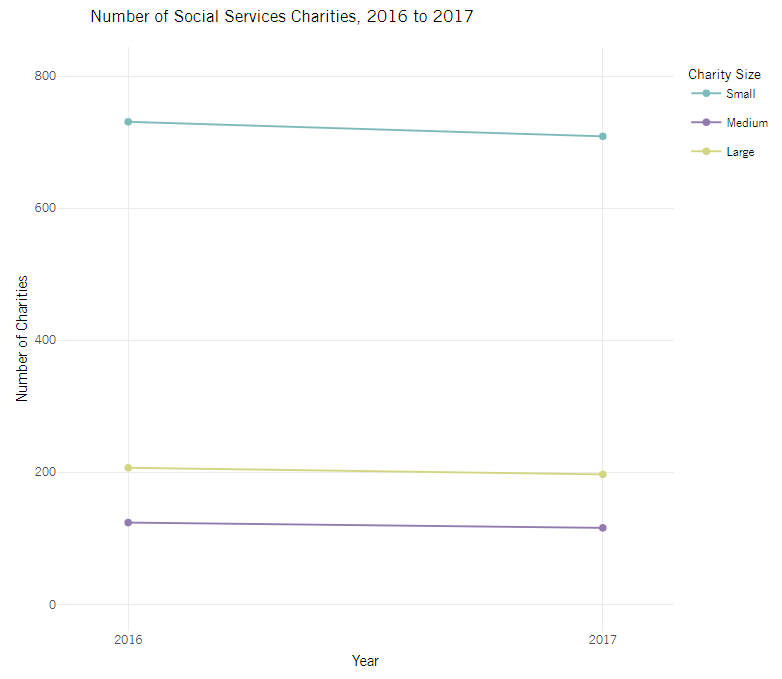
\includegraphics{Fig2 SocServ Charity Size.png}
\caption{Count of Social Services Charities by Charity Size}
\end{figure}

The majority of Victoria's social service charities were small charities (731 charities in 2016, 709 in 2017), followed by large charities (207 in 2016, 197 in 2017) and medium-size charities (124 in 2016 and 116 in 2017).

Figure 3 shows that most community service organisations (including social service charities) had no change or slight decrease in numbers. Only other education organizations and economic, social and community development organizations had a growth from 2016 to 2017.

\begin{figure}
\centering
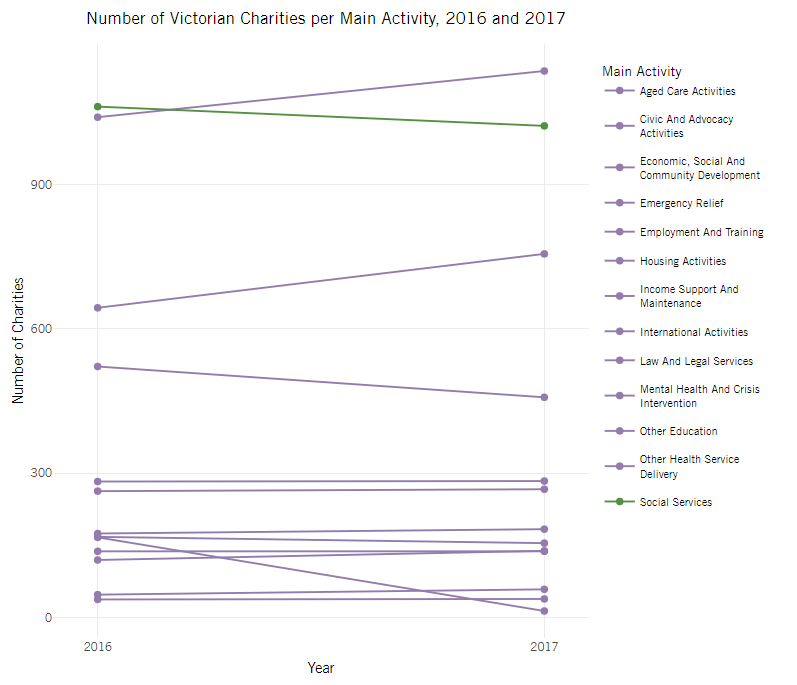
\includegraphics{Fig3 Main Activity.png}
\caption{Count of Victorian Charities per Main Activity}
\end{figure}

\hypertarget{workforce-composition}{%
\subsection{Workforce Composition}\label{workforce-composition}}

The charitable services sector is a large and growing employer. Analysis of the ACNC 2016-2017 data show that Victorian social service industry employed 35,296 people in 2016 and this figure was increased to 43,697 in 2017.

From 2016 to 2017, the dominant staff type in social service sector was changed from part-time to full-time. The number of casual staff was the smallest in 2016 and 2017 compared with other staff types. A slight decrease in number of casual employees was seen in the period of 2016 to 2017; from 8,258 to 8,222 respectively. There were changes in the number of part-time employees and the number of full-time employees as well. The number of part-time employees decreased from 15,220 to 14,570 and the number of full-time employees was increased from 11,818 to 20,905.

\begin{figure}
\centering
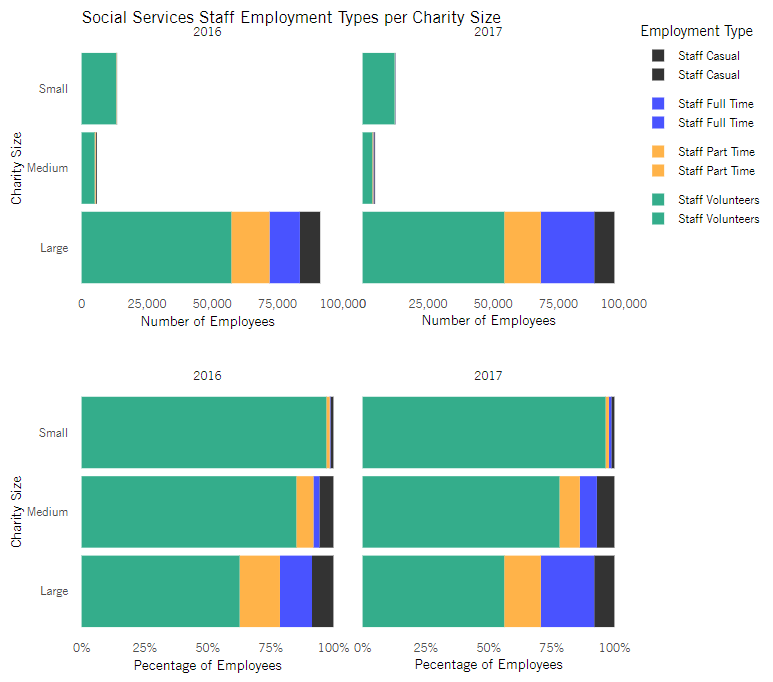
\includegraphics{Fig4 CharSize EmployType.PNG}
\caption{Number of Workers in the Social Services Industry by Organisation Size and Employment Status}
\end{figure}

Large charities employed around 96\% of social services industry workers in Victoria in 2016 and 2017.
This comprised:

\begin{itemize}
\tightlist
\item
  11,635 and 20,456 full-time workers (34.2\% and 48.5\%)
\item
  14,644 and 14,014 part-time workers (43\% and 33.2\%)
\item
  7,773 and 7,734 casual workers (22.8\% and 18.3\%)
\end{itemize}

Medium-size charities employed around 2.4\% of the total social service industry workforce in 2016 and 2017. The medium-size charity workforce comprised:

\begin{itemize}
\tightlist
\item
  139 and 325 full-time workers (16.1\% and 31.1\%)
\item
  398 and 387 part-time workers (45.1\% and 37\%)
\item
  326 and 334 casual workers (37.8\% and 31.9\%)
\end{itemize}

Small charities employed around 1\% of the total social service industry workforce in 2016 and 2017. The small charity workforce comprised:

\begin{itemize}
\tightlist
\item
  44 and 124 full-time workers (11.5\% and 27.7\%)
\item
  178 and 169 part-time workers (46.7\% and 37.8\%)
\item
  326 and 334 casual workers (41.7\% and 34.4\%)
\end{itemize}

The vast majority of Victorian Social services industry charities are supported by unpaid volunteer worker. Volunteer workers accounts for 68.2\% of the total social service industry workforce in 2016 and was decreased slightly to 61.7\%.

Small charities of social service sectors rely the most on volunteers (97.2\% in 2016, 96.5\% in 2017) followed by medium (85.3\% and 78.2\%) and large charities (62.7\% and 56.3\%).

In other comunity service sectors, Civic and advocacy activites had the most volunteers in 2016 but had a huge drop from 77403 to 620 in 2017. In 2017, other education sectors got the highest numbers of volunteers. Social services were in the second place in both years and had a slightly decreasing from 75,605 to 70,289 people.

\hypertarget{sector-funding}{%
\subsection{Sector Funding}\label{sector-funding}}

The Victorian social services industry collectively received an income of around \$3 billion in 2016 and
\$2.3 billion in 2017 with around 60\% these generated from government grants.\\
Social services industry received the most in government grants (\$2.1bn and \$1.97bn) in 2016 and 2017, with other health service delivery second (\$1.6bn) in 2016 and aged care service delivery second (\$1.5bn) in 2017. International activities raised the most from donations and bequests (\$513m and \$438m).\\
Figure 5 shows government grants are the single biggest source of income for Victorican social service charities. All other income and revenue combined raised nearly \$650m for social service charities but the amount was decreased substantially to \$180m by 2017, while donations and bequests raised over \$200m in each year.

\begin{figure}
\centering
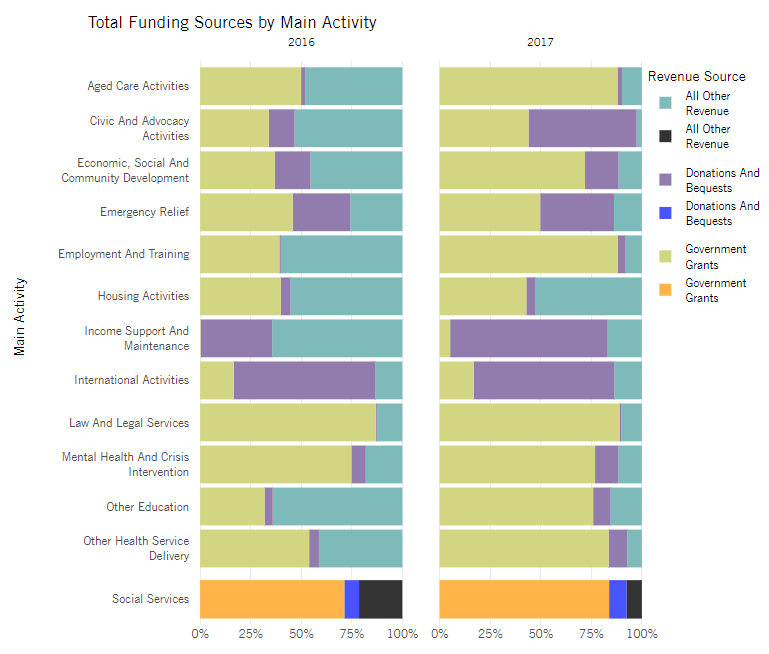
\includegraphics{Fig5 Funding Props.PNG}
\caption{Proportion of Funding Sources per Main Activity}
\end{figure}

Large social service charities received most money from government grants, which was around \$2 billion. Income from donations and bequests decreased from \$200m to \$184m while other income and revenue received decreased from \$600m to \$158m in 2016-2017.\\
Medium-sized social service charities raised \$14m in other income and revenue in 2017, a decrease from the previous year. They also raised around \$10m in donations and bequests, a slight decrease from the previous year. Reported income from government grants was \$17m, which was a slight decrease from 2016.\\
Small social service charities received just around \$5m in other income and revenue, little change from 2016. They also raised \$7.3m from donations and bequests, a slight increase from \$7.1m in the previous year. Small social service charities also received around \$3.9m from government grants, almost the same as the previous year.

\hypertarget{financial-health-of-sector}{%
\subsection{Financial Health of Sector}\label{financial-health-of-sector}}

The financial health of social service charities affects their ability to deliver vital services to people facing disadvantage. Figure 6 shows the majority of Victorian social service charities (539 in 2016 and 537 in 2017) were in budget surplus. 82 social service charities operated a balanced budget in 2017 and this is a decrease on the number of charities from the previous year. 403 charites were in deficit in 2017 and it was changed little from the previous year.

\begin{figure}
\centering
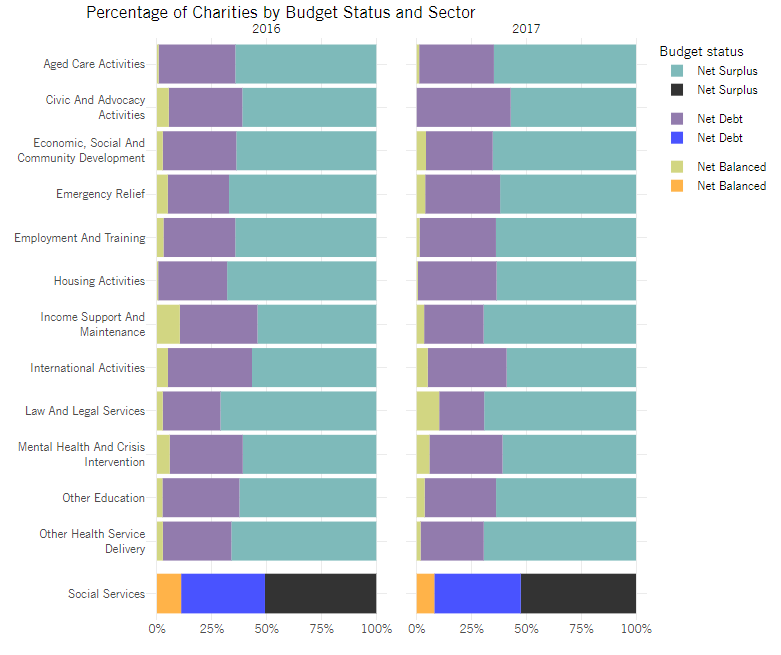
\includegraphics{Fig6 Budget Status props.PNG}
\caption{Budget status per Main Activity}
\end{figure}

Small social service charities were more likely to operate budget deficits and a balanced budged than medium-sized and large charities. Around 43.6\% of small charities operated budget deficits, compared to 21.7\% of large organisations and 33.9\% of medium-sized organisations in 2016. Figures changed to 44\%, 24.9\% and 31.9\% respectively in 2017.\\
Around 40.9\% of small charities in 2016 and 44\% in 2017 operated budget surplus compared to 77.8\% and 75.1\% of large charities and 63.7\% and 66.4\% of medium-sized charities. Conversely, 15.5\%/11.3\% of small charities operated in a balanced budget, compared to 2.4\%/2.7\% of medium-sized organisations and 0.5\%/0\% of large charities.\\
Charities whose main activity was law and legal services were more likely to operate budget surpluses in 2016 while Charities whose main activity was income support and maintenance were more likely in 2017. Charities whose main activity was international activities were most likely to operate budget deficits in 2016 but in 2017 civic and advocacy activities charities got the highest chance of budget deficits. Charities whose main activity was social service were most likely to have balanced budgets in 2016 but law and legal service charities became more likely in 2017.

\hypertarget{discussion}{%
\section{Discussion}\label{discussion}}

This report visualised the 2016 and 2017 ACNC datasets for Victoria charities and not-for-profit organisations, which is a strong and fast growing industry, particularly the social services industry. Social services industry is a key component of Victorian economy and also a key employer. It consists of thousands of charities, employing tens of thousands of staff and having thousands of volunteers. It is a billion dollar sector receiving a large amount of income from governments, donations and other revenue (eg. Service fees). The financial support from government contributes to the growth of the sector.\\
As the charitable and not-for-profit social services sector is so large and the nature of the data is a summary of surveyed reportings, it was necessary that analysis of the data began with exploratory techniques in the form of visualisations.

\hypertarget{interpretation-of-results}{%
\subsection{Interpretation of Results}\label{interpretation-of-results}}

\hypertarget{social-services-sector-size-1}{%
\subsubsection{Social Services Sector Size}\label{social-services-sector-size-1}}

Considering the large contribution to essential services provided by the charities in the social services sector such as aged care, disability care, etc, it was expected that socials services charities would make up a large proportion of all charities operating in Victoria. However, the finding that social services charities comprised more than 1 out of 5 Victorian charities in 2016 and 2017 highlighted the important contribution that charities make to social services.\\
Considering the large quantity of charities performing social services, it was expected that a similarly large proportion of social services charities were small or medium in size. The number of large social services charities was greater than medium-sized charities for both 2016 and 2017, which could be due to the nature of the social services provided. This could be in the form that larger charities tend to provide social services such as aged care and disability care, while smaller charities provide more specialised social services like Returned Soldiers Leagues for individual communities/suburbs and individual childcare facilities.

\hypertarget{workforce-composition-1}{%
\subsubsection{Workforce Composition}\label{workforce-composition-1}}

It was also unsurprising that charities in the social services sector employed a very large number of paid staff and volunteers throughout the years, but the visualisations revealed such a large proportion of the total workforce are employed by large charities. The visualisations also revealed that the number of volunteers working in social services charities outweighed the total number of paid staff across both years, underlining the sector's reliance on unpaid staff. When focusing on medium and smaller charities, not only do volunteers comprise the majority of staff, but they are often more than 90\% of the total staff count in social services charities of these sizes.

\hypertarget{sector-funding-1}{%
\subsubsection{Sector Funding}\label{sector-funding-1}}

Government grants are the majority of funding sources for charities and not-for-profits across all but one sector (international activities), and charities in the social services sector are no exception. Charities operating in social services collected the greatest amount of government grants in both 2016 and 2017, which shows how much the sector is reliant on government funding to perform their services. Furthermore, large social services charities received approximately three quarters (75\%) of their total funding from government grants in each year, which was in contrast to small and medium social charities that received smaller proportions of their funding from government grants. Large social services charities also received a much greater proportion of their funding from government grants than large charities in other sectors, which only further emphasises the reliance on government funding to maintain social services.

\hypertarget{financial-health-of-sector-1}{%
\subsubsection{Financial Health of Sector}\label{financial-health-of-sector-1}}

\hypertarget{method-of-analysis}{%
\subsection{Method of Analysis}\label{method-of-analysis}}

\hypertarget{limitations-and-improvements}{%
\subsection{Limitations and Improvements}\label{limitations-and-improvements}}

The data used in this report is sourced from Annual Information Statements (AIS) collected by the ACNC from registered charities categorised as charities and not-for-profit organisations. The reasons for changes in social services sector include:

\begin{itemize}
\tightlist
\item
  Changes in numbers of charities registered with the ACNC
\item
  Main activity of charities are changed which may explain the big increase in the number of social services charities
\item
  More charities completed and submitted the AIS before due date
\end{itemize}

While the report gives a detailed visualization of the data set, there still need improvements in .

\hypertarget{summary}{%
\subsection{Summary}\label{summary}}

\newpage
\setstretch{1.25}
\onecolumn

\hypertarget{references}{%
\section{References}\label{references}}

\fontsize{11}{14}

\begin{itemize}
\item
  Australian Association of Social Workers, 2020, \emph{What is social work?}, AASW - Australian Association of Social Workers, accessed 11/04/2020, \url{https://www.aasw.asn.au/information-for-the-community/what-is-social-work}
\item
  Australian Charities and Not-For-Profit Commission, \emph{Australian Charities Report 2017}, accessed 21/04/2020, \url{https://www.acnc.gov.au/tools/reports/australian-charities-report-2017}
\item
  Australian Institute of Health and Welfare, 2018, \emph{Older Australia at a glance}, accessed 12/04/2020, \url{https://www.aihw.gov.au/reports/older-people/older-australia-at-a-glance/contents/demographics-of-older-australians/australia-s-changing-age-and-gender-profile}
\item
  Berinato, S, Visualizations That Really Work, Harvard Business Review, 92-100, June 2016
\item
  Brown, M., 2020, \emph{Intellectually disabled people `unsafe' in hospitals, disability royal commission hears}, ABC News, Australia, \url{https://www.abc.net.au/news/2020-02-25/hospitals-not-safe-for-intellectually-disabled-inquiry-told/11999170}
\item
  Karanasios, S., 2018, \emph{Chapter Six: Information sharing and technological innovation}, Victorian Council of Social Services, accessed 18/04/2020, \url{http://vcoss.org.au/wp-content/uploads/2018/02/Community-services-of-the-future-FSSI-2018-FINAL.pdf}
\item
  Department of Social Services, 2019, \emph{Our Responsibilities}, Australian Government, accessed 10/04/2020, \url{https://www.dss.gov.au/our-responsibilities}
\item
  Department of Health and Social Services, 2020, *Our Services, Victorian Government, accessed 10/04/2020, \url{https://www.dhhs.vic.gov.au/our-services}
\item
  Dew, A., Gilroy, J., \& Lincoln, M., 2016, \emph{A Sustainable Rural and Remote Workforce for Disability: Research to Action Guide}, Rapid Review, Centre for Applied Disability Research
\item
  Fielding, N.G., Lee, R.M. and Blank, G. (2016). The SAGE Handbook of Online Research Methods. {[}online{]} Google Books. SAGE. Available at: \url{https://books.google.com.au/books?hl=en\&lr=\&id=IMWCDQAAQBAJ\&oi=fnd\&pg=PA307\&dq=data+visualisation+\&ots=79d-fEIGUD\&sig=M3xpg9xl0oNSrqa_T9aK6FIWZR4\&redir_esc=y\#v=onepage\&q\&f=false} {[}Accessed 17 Apr.~2020{]}.
\item
  Glanz, D., 2016, \emph{RMIT is hosting a new research and teaching institute that puts Victoria in the box seat ahead of significant change in the delivery of social service.}, Royal Melbourne Institute of Technology, accessed 10/04/2020, \url{https://www.rmit.edu.au/news/all-news/2016/june/rmit-to-host-social-service-institute}
\item
  Hutchens, G., 2018, \emph{Scott Morrison announces royal commission into aged care after string of scandals}, The Guardian Australia, accessed 12/04/2020, \url{https://www.theguardian.com/australia-news/2018/sep/16/morrison-to-announce-royal-commission-into-aged-care-after-string-of-scandals}
\item
  International Federation of Social Workers, 2014, \emph{GLOBAL DEFINITION OF SOCIAL WORK}, accessed 11/04/2020, \url{https://www.ifsw.org/what-is-social-work/global-definition-of-social-work/}
\end{itemize}

\newpage

\begin{itemize}
\item
  Kyle, L., Macdonald, F., Bentham, E., 2018, \emph{CHAPTER FOUR - Workforce of the future for Community Services Industry Plan}, Victorian Council of Social Services, \textbf{Community services of the future, An evidence review}, accessed 19/04/2020, \url{http://vcoss.org.au/wp-content/uploads/2018/02/Community-services-of-the-future-FSSI-2018-FINAL.pdf}
\item
  McKenzie, N., Baker, R., 2014, \emph{Abusive and corrupt staff employed by Yooralla despite warnings, leaked documents and whistleblowers claim}, The Age, Victoria Australia, accessed 21/04/2020, \url{https://www.theage.com.au/national/abusive-and-corrupt-staff-employed-by-yooralla-despite-warnings-leaked-documents-and-whistleblowers-claim-20141123-11s5wa.html}
\item
  McKinsey Global Institute, 2017, *Briefing note for the Fortune Vatican Forum December 2016, McKinsey and Company, \url{https://www.scribd.com/document/354361488/MGI-Futureof-Work-Briefing-Note-May-2017}
\item
  National Disability Insurance Scheme, 2020, \emph{What is the NDIS?}, accessed 12/04/2020, \url{https://www.ndis.gov.au/understanding/what-ndis}
\item
  \emph{National Disabliity Insurance Scheme Act 2013}, \url{https://www.legislation.gov.au/Details/C2013A00020}
\item
  Royal Commission into Aged Care Quality and Safety, 2018, \emph{Terms of Reference}, accessed 12/04/2020, \url{https://agedcare.royalcommission.gov.au/Pages/Terms-of-reference.aspx}
\item
  Polack, N. (2019). NHS Scotland Open Data: A data visualisation study about child health. {[}online{]} Available at: \url{http://www.cs.stir.ac.uk/courses/msc/projects/PastProjects/exemplars/Natalie_Polack.pdf} {[}Accessed 18 Apr.~2020{]}.
\item
  PolicyMap. (n.d.). PolicyMap. {[}online{]} Available at: \url{https://www.policymap.com/} {[}Accessed 18 Apr.~2020{]}.
\item
  Prime Minister, Minister for Families and Social Services, 2019, \emph{ESTABLISHMENT OF THE ROYAL COMMISSION INTO VIOLENCE, ABUSE, NEGLECT AND EXPLOITATION OF PEOPLE WITH DISABILITY}, accessed 21/04/2020, \url{https://www.pm.gov.au/media/establishment-royal-commission-violence-abuse-neglect-and-exploitation-people-disability}
\item
  United Nations (2015), \emph{World's Women: Trends and Statistics 2015}, United Nations, New York
\item
  Young, J. and Wessnitzer, J. (2016). Descriptive Statistics, Graphs, and Visualisation. Human-Computer Interaction Series, pp.37-56.
\end{itemize}

\newpage

\hypertarget{appendices}{%
\section{Appendices}\label{appendices}}

\hypertarget{appendix-1-guiding-questions}{%
\subsection{Appendix 1: Guiding Questions}\label{appendix-1-guiding-questions}}

\begin{itemize}
\tightlist
\item
  Are some types of organisations categorised as community services growing more quickly than others?
\item
  Has there been a change in the size of organisations over time? Has the proportion of small to large sized organisations changed or remained constant? Is the change more apparent among some types of organisations?
\item
  How many workers are employed in the community services industry? What is the breakdown of part-time/full-time/casual? Can we get this data by type of organisation? Are the proportions of casual and part-time employees growing faster in some types or sizes of organisations than others?
\item
  Has the number of volunteers or - who they are employed by - changed over time?
\item
  What proportion of services are providing NDIS services? Has this changed since 2017? Are large or small organisations more likely to provide NDIS services?
\item
  Has there been a change in the source of income for community service organisations? Is this change more apparent by organisation size or type?
\item
  Is the proportion of income being spent on employee expenses changing or remaining constant?
\item
  What size or type of organisations are most likely to have a deficit budget?
\end{itemize}

\newpage

\hypertarget{appendix-2-acnc-datasets}{%
\subsection{Appendix 2: ACNC Datasets}\label{appendix-2-acnc-datasets}}

The 2017 ACNC data set was sourced from the following data.gov.au website:\\
\textbf{\url{https://data.gov.au/dataset/ds-dga-a1f8626c-fefb-4c4d-86ea-deaa04fb1f6e/details?q=}}.\\
This data was cleaned and filtered to VCOSS standards to ensure consistency with the 2016 dataset that was supplied by VCOSS. The below details are the requirements set out by VCOSS for cleaning.

\includegraphics[width=\textwidth,height=0.85\textheight]{../../VCOSS ACNC Data Cleaning Guidelines p1.pdf}

\includegraphics[width=\textwidth,height=0.85\textheight]{../../VCOSS ACNC Data Cleaning Guidelines p2.pdf}

\newpage

\hypertarget{appendix-3-identifying-invalid-abns}{%
\subsection{Appendix 3: Identifying Invalid ABNs}\label{appendix-3-identifying-invalid-abns}}

\begin{Shaded}
\begin{Highlighting}[]
\CommentTok{# Removing Invalid ABNs}

\CommentTok{## Reference Keybreaker file}

\NormalTok{ABN_Keybreaker <-}\StringTok{ }\KeywordTok{read_excel}\NormalTok{(}\StringTok{"VCOSS Data/ABN Keybreaker.xlsx"}\NormalTok{)}

\KeywordTok{datatable}\NormalTok{(ABN_Keybreaker,}
          \DataTypeTok{class =} \StringTok{"compact"}\NormalTok{,}
          \DataTypeTok{options =} \KeywordTok{list}\NormalTok{(}\DataTypeTok{pageLength =} \DecValTok{11}\NormalTok{,}
                         \DataTypeTok{searching =} \OtherTok{FALSE}\NormalTok{,}
                         \DataTypeTok{lengthChange =} \OtherTok{FALSE}\NormalTok{))}
\CommentTok{## Function for checking ABNs}

\NormalTok{ABN_Checker <-}\StringTok{ }\ControlFlowTok{function}\NormalTok{(ABN_No) \{}
  
\NormalTok{  sumproduct <-}\StringTok{ }\KeywordTok{c}\NormalTok{()}
  
  \ControlFlowTok{for}\NormalTok{(position }\ControlFlowTok{in} \DecValTok{1}\OperatorTok{:}\KeywordTok{nchar}\NormalTok{(ABN_No)) \{}
    
\NormalTok{    number <-}\StringTok{ }\KeywordTok{as.numeric}\NormalTok{(}\KeywordTok{substr}\NormalTok{(ABN_No, position, position))  }
    
    \ControlFlowTok{if}\NormalTok{(position }\OperatorTok{==}\StringTok{ }\DecValTok{1}\NormalTok{) \{}
      
\NormalTok{      number <-}\StringTok{ }\KeywordTok{as.numeric}\NormalTok{(number }\OperatorTok{-}\StringTok{ }\DecValTok{1}\NormalTok{)}
      
\NormalTok{    \}}
    
\NormalTok{    product <-}\StringTok{ }\NormalTok{(number }\OperatorTok{*}\StringTok{ }\NormalTok{ABN_Keybreaker}\OperatorTok{$}\NormalTok{Weighting[position])}
    
\NormalTok{    sumproduct <-}\StringTok{ }\KeywordTok{sum}\NormalTok{(sumproduct, product)}
    
\NormalTok{  \}}
  
  \ControlFlowTok{if}\NormalTok{(sumproduct }\OperatorTok\StringTok{ }\DecValTok{89} \OperatorTok{==}\StringTok{ }\DecValTok{0}\NormalTok{) \{}
    
\NormalTok{    Check <-}\StringTok{ "Valid ABN"}
    
\NormalTok{  \} }\ControlFlowTok{else}\NormalTok{ \{}
    
\NormalTok{    Check <-}\StringTok{ "Invalid ABN"}
    
\NormalTok{  \}}
  
  \KeywordTok{return}\NormalTok{(Check)}
  
\NormalTok{\}}

\NormalTok{ABN_Validator <-}\StringTok{ }\ControlFlowTok{function}\NormalTok{(ABN_vector) \{}
  
  \KeywordTok{sapply}\NormalTok{(ABN_vector, ABN_Checker)}
  
\NormalTok{\}}



\NormalTok{VCOSS_ACNC_}\DecValTok{16}\NormalTok{ <-}\StringTok{ }\KeywordTok{mutate}\NormalTok{(VCOSS_ACNC_}\DecValTok{16}\NormalTok{,}
                        \DataTypeTok{ABN_Validation =} \KeywordTok{ABN_Validator}\NormalTok{(abn))}

\NormalTok{Invalid_ABNs_}\DecValTok{16}\NormalTok{ <-}\StringTok{ }\KeywordTok{filter}\NormalTok{(VCOSS_ACNC_}\DecValTok{16}\NormalTok{,}
\NormalTok{                          ABN_Validation }\OperatorTok{==}\StringTok{ "Invalid ABN"}\NormalTok{)}

\NormalTok{VCOSS_ACNC_}\DecValTok{17}\NormalTok{ <-}\StringTok{ }\KeywordTok{mutate}\NormalTok{(VCOSS_ACNC_}\DecValTok{17}\NormalTok{,}
                        \DataTypeTok{ABN_Validation =} \KeywordTok{ABN_Validator}\NormalTok{(abn))}

\NormalTok{Invalid_ABNs_}\DecValTok{17}\NormalTok{ <-}\StringTok{ }\KeywordTok{filter}\NormalTok{(VCOSS_ACNC_}\DecValTok{17}\NormalTok{,}
\NormalTok{                          ABN_Validation }\OperatorTok{==}\StringTok{ "Invalid ABN"}\NormalTok{)}


\CommentTok{## Filter out invalid ABNs from VCOSS dataframes}

\NormalTok{VCOSS_ACNC_}\DecValTok{16}\NormalTok{ <-}\StringTok{ }\NormalTok{VCOSS_ACNC_}\DecValTok{16}\NormalTok{[}\KeywordTok{which}\NormalTok{(}\OperatorTok{!}\NormalTok{(VCOSS_ACNC_}\DecValTok{16}\OperatorTok{$}\NormalTok{abn }\OperatorTok\StringTok{ }\NormalTok{Invalid_ABNs_}\DecValTok{16}\OperatorTok{$}\NormalTok{abn)), ]}

\NormalTok{VCOSS_ACNC_}\DecValTok{17}\NormalTok{ <-}\StringTok{ }\NormalTok{VCOSS_ACNC_}\DecValTok{17}\NormalTok{[}\KeywordTok{which}\NormalTok{(}\OperatorTok{!}\NormalTok{(VCOSS_ACNC_}\DecValTok{17}\OperatorTok{$}\NormalTok{abn }\OperatorTok\StringTok{ }\NormalTok{Invalid_ABNs_}\DecValTok{17}\OperatorTok{$}\NormalTok{abn)), ]}
\end{Highlighting}
\end{Shaded}

\end{document}
